%!TEX program = xelatex
%!TEX options=--shell-escape
\documentclass[12pt]{article}

%
\usepackage[scheme=plain]{ctex}
%
\usepackage{fontspec}
%
\usepackage[margin = 1in]{geometry}

%
\usepackage[dvipsnames]{xcolor}
\usepackage[many]{tcolorbox}

%
\usepackage{amsmath}
\usepackage{amssymb}
\usepackage{amsthm}
%
\usepackage{tensor}
%
\usepackage{slashed}
\usepackage{physics}
\usepackage{simpler-wick}

%
\usepackage[version=4]{mhchem}

%
\usepackage{mathtools}

%
\usepackage{bm}
\newcommand{\dbar}{\dif\hspace*{-0.18em}\bar{}\hspace*{0.2em}}
\DeclareMathAlphabet\mathbfcal{OMS}{cmsy}{b}{n}
%\usepackage{bbold}
\newcommand*{\dif}{\mathop{}\!\mathrm{d}}
\newcommand*{\euler}{\mathrm{e}}
\newcommand*{\imagi}{\mathrm{i}}

\renewcommand{\vec}[1]{\boldsymbol{\mathbf{#1}}}

\usepackage{caption}
\usepackage{multirow}
\usepackage{enumitem}

%
\usepackage{mathrsfs}
\usepackage{dsfont}

%
\usepackage{hyperref}
\hypersetup{
    colorlinks=true,
    linkcolor=violet,
    filecolor=blue,      
    urlcolor=blue,
    citecolor=cyan,
}

%
\usepackage{graphicx}
\usepackage{subfig}
%
\graphicspath{{figures/}{../figures/}}


%
\usepackage{indentfirst}
%
\setlength{\parindent}{2em}
\linespread{1.25}

% 
% \setmainfont{Times New Roman}

\title{Note}
\author{Feng-Yang Hsieh}
\date{}

\begin{document}
\maketitle

\section{CWoLa}% (fold)
\label{sec:cwola}
	The Classification Without Labels (CWoLa) is a weakly supervised learning method. The CWoLa approach trains a model to discriminate the mixed samples, which are mixtures of the original signal and background samples. The optimal classifier in the CWoLa approach is also the optimal classifier in the traditional fully-supervised case where all label information is available. This section utilizes the CWoLa approach to train classifiers on di-Higgs samples.

	\subsection{Sample}% (fold)
	\label{sub:sample}
		In this exercise, the signal corresponds to the resonant Higgs boson pairs production in the four-$b$ quarks channel. These Higgs boson pairs are produced via gluon-gluon fusion in the two Higgs doublet model (2HDM). The Higgs boson $h$ ($m_h = \text{125 GeV}$) pair is produced by the heavy CP-even scalar $H$ with mass $m_H$ ranging from $\text{300 GeV}$ to $\text{1200 GeV}$. The background consists of QCD multi-jet events.

		The CWoLa training samples $M_1$ and $M_2$ are the mixtures of the signal and background samples. The probability distribution of the mixed sample is a combination of the signal $p_s(x)$ and background $p_B(x)$ distributions:
		\begin{equation}
			\begin{aligned}
				p_{M_1}(x) &=  f_1 p_S(x) + (1-f_1) p_B(x) \\
				p_{M_2}(x) &=  f_2 p_S(x) + (1-f_2) p_B(x)
			\end{aligned}
		\end{equation}
		where $f_1, f_2$ are the signal fractions, and $x$ represents the observables used for the classification task.

		DNN and SPANet network architectures are considered in this exercise. For DNN, the input features are summarised in Table \ref{tab:DNN_variables}, consisting of 16 variables. For SPANet, the input features are a list of final jets, each represented by their 4-momentum $(p_\text{T}, \eta,\phi, M)$ and a boolean $b$-tag.
		\begin{table}[htpb]
			\centering
			\caption{Input variables used to train the dense neural network.}
			\label{tab:DNN_variables}
			\begin{tabular}{l|c|c}
				Reconstructed objects       & Variables used for training   & \# \\ \hline
				Higgs candidate             & $(p_\text{T}, \eta, \phi, m)$ & 8  \\
				Subjets                     & $\Delta R(j_1,j_2)$                    & 2  \\
				b-tagging                   & Boolean for $j_i \in h_{1,2}^{\text{cand}}$       & 4  \\
				Di-Higgs system             & $p_\text{T}^{hh}, m_{hh}$        & 2 
			\end{tabular}		
		\end{table}

	% subsection sample (end)
	\subsection{Result}% (fold)
	\label{sub:result}
		The CWoLa training utilizes samples with different signal fractions $f_1,f_2$ to train the classifiers. The results of CWoLa training are shown in Figure~\ref{fig:CWoLa_training_result} with different signal fractions. When $f_1$ is far from $0.5$, the results tend to approach those of the fully supervised case.
		\begin{figure}[htpb]
			\centering
			\subfloat[DNN]{
				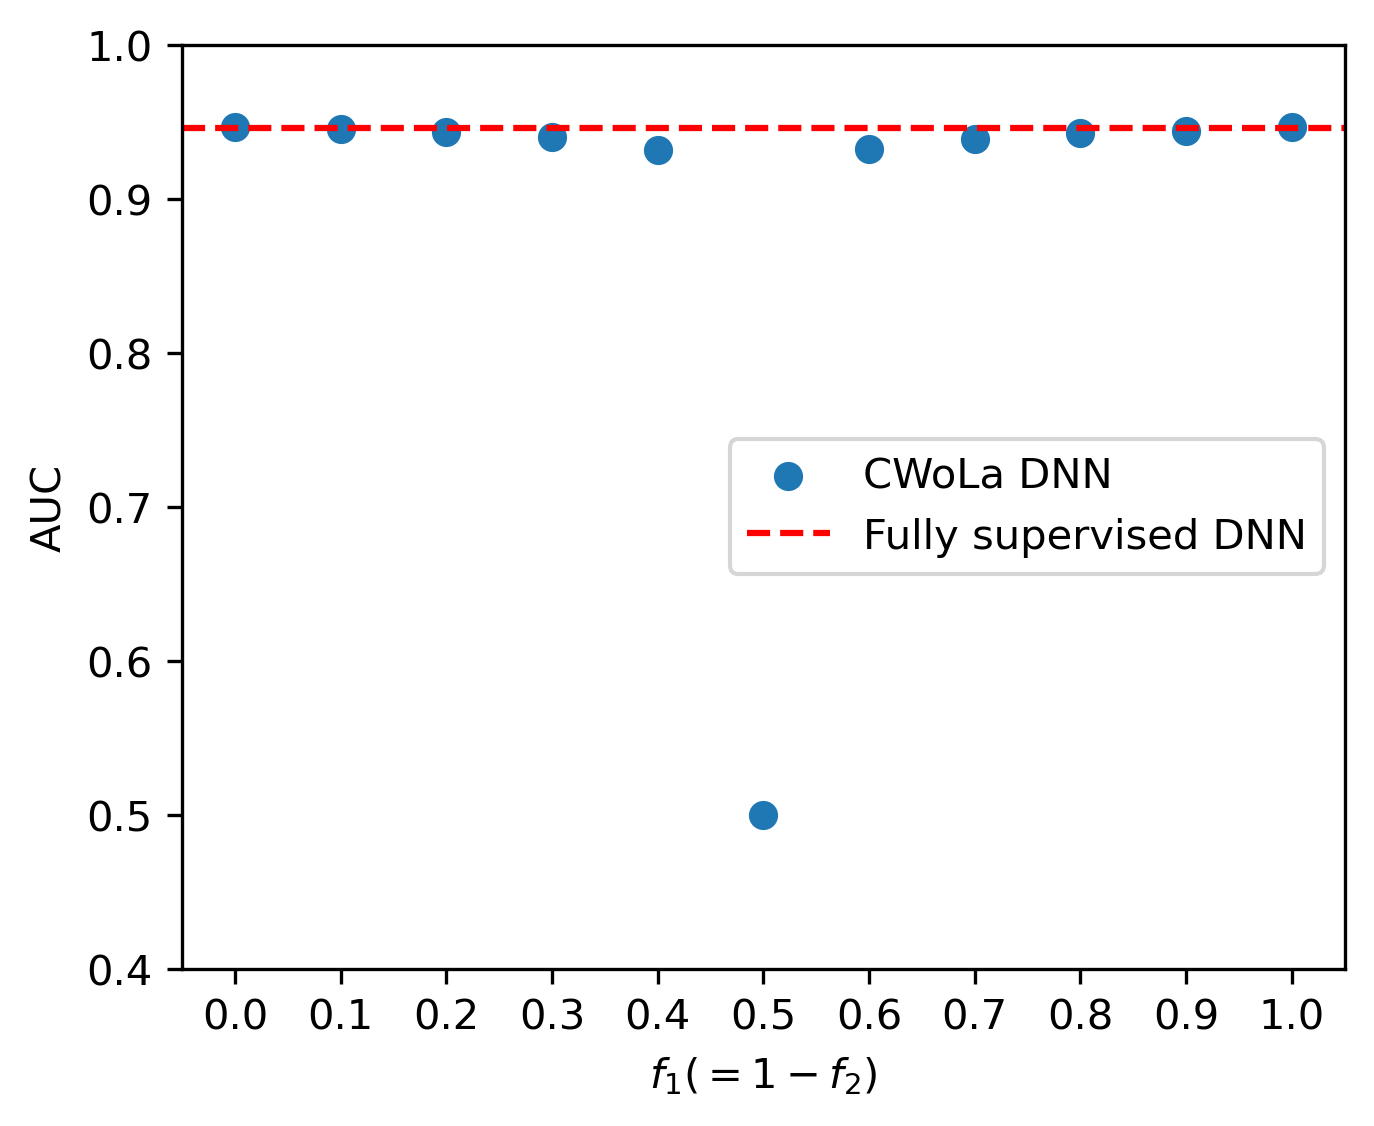
\includegraphics[width=0.45\textwidth]{CWoLa_DNN.png}
			}
			\subfloat[SPANet]{
				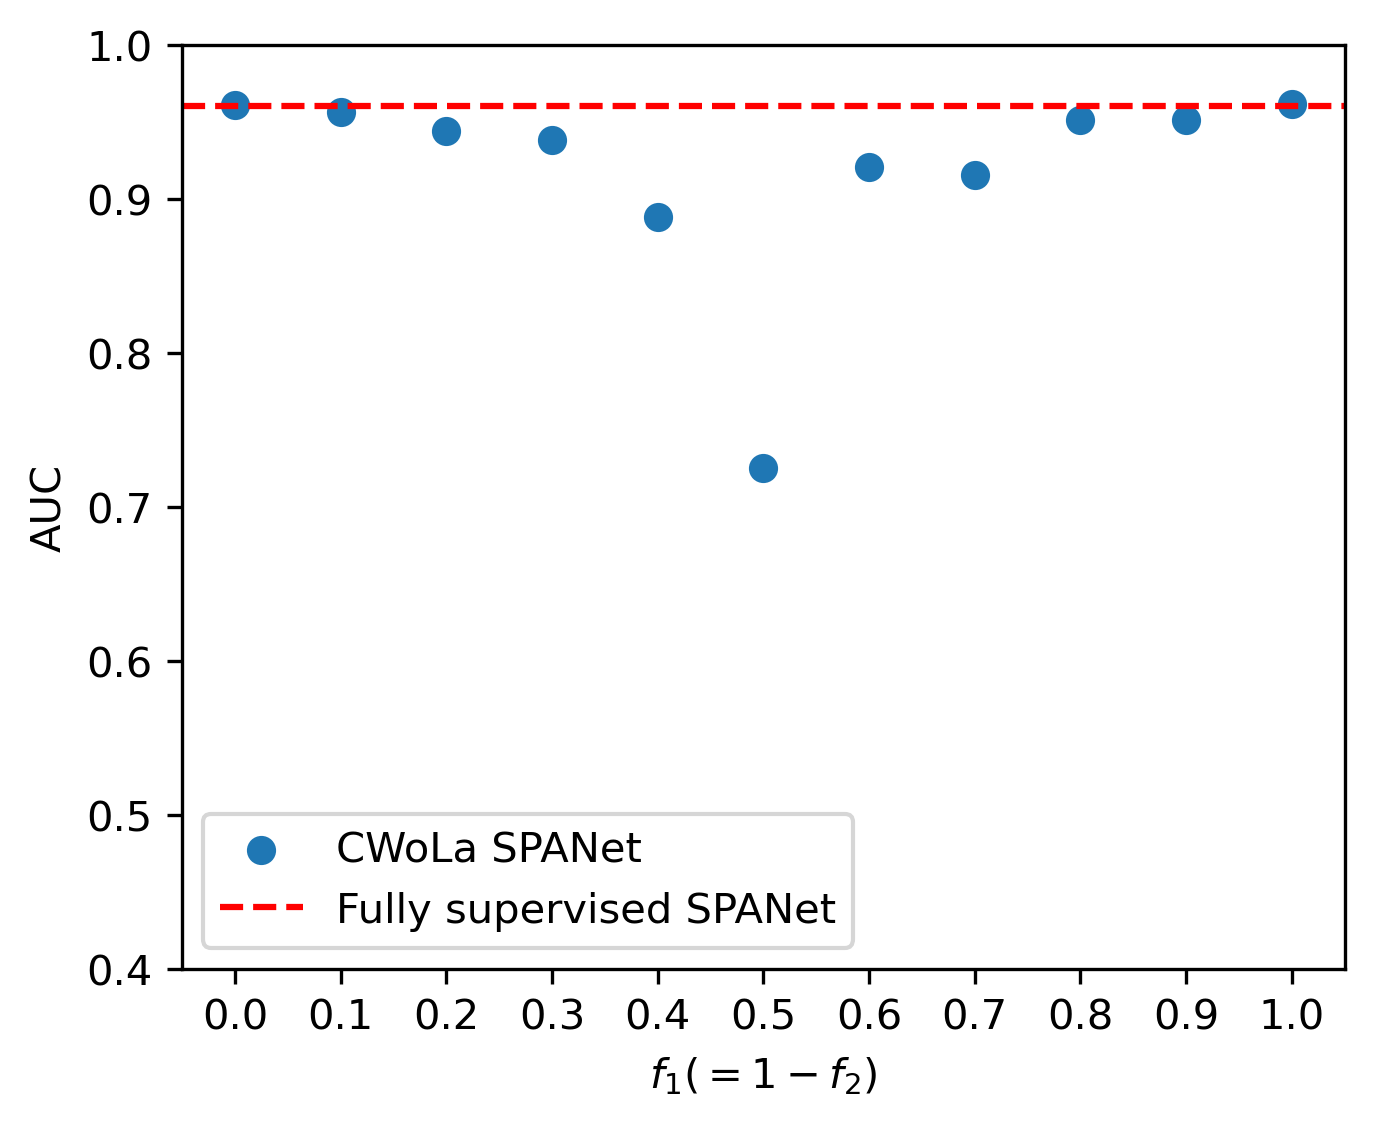
\includegraphics[width=0.45\textwidth]{CWoLa_SPANet.png}
			}
			\caption{The AUC of CWoLa training as a function of the signal fraction $f_1$. For simplicity, we set signal fraction $f_2$ equal to $1 - f_1$. The horizontal dashed line indicates the fully-supervised AUC.}
			\label{fig:CWoLa_training_result}
		\end{figure}

		When $f_1 = 0.5$ the mixed sample $M_1$ and $M_2$ have identical distributions, so the classifier can not learn anything in this case. In the case of DNN, the AUC is $0.5$, as expected. However, for SPANet, the AUC is more than $0.7$.

		This is because SPANet is trained on both pairing and classification tasks simultaneously. The pairing part introduces some asymmetries between signal and background samples, leading to the AUC that deviates from $0.5$.

		To investigate the effect of the pairing task on SPANet's performance, the weight of the pairing component is set to zero, meaning that SPANet focuses solely on the classification task. Figure~\ref{fig:CWoLa_SPANet_without_pairing} shows the SPANet training results without pairing task. In this case, as expected, the AUC is close to $0.5$ when $f_1 = 0.5$. 
		\begin{figure}[htpb]
			\centering
			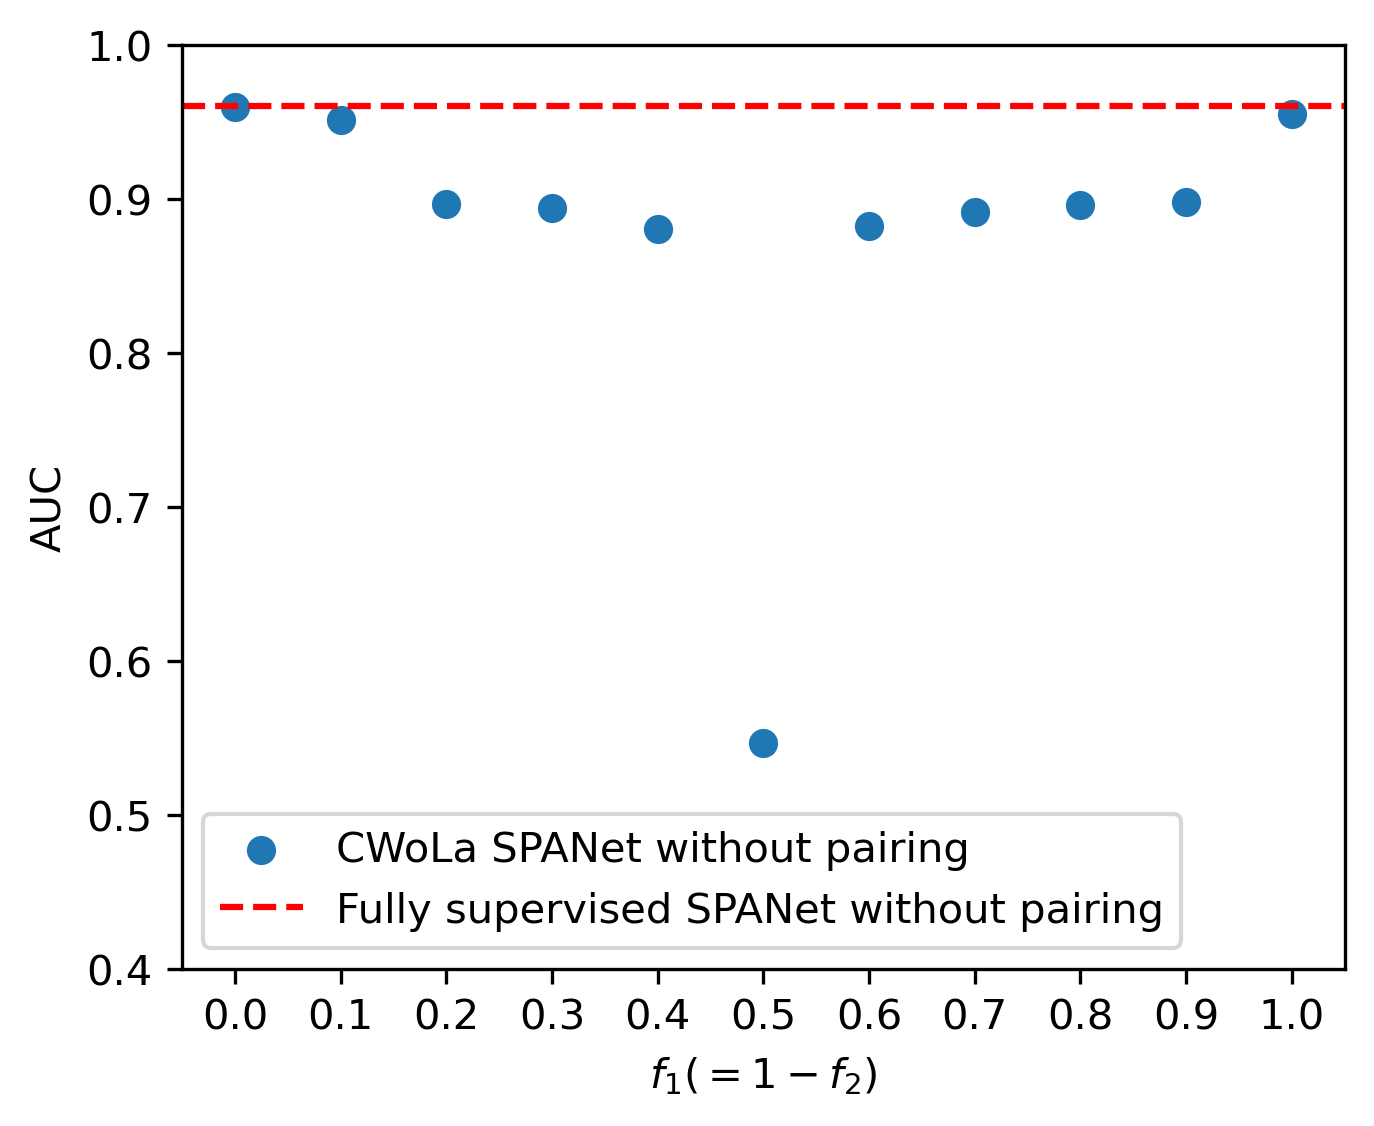
\includegraphics[width=0.45\textwidth]{CWoLa_SPANet_no_pair.png}
			\caption{The AUC of CWoLa SPANet training as a function of the signal fraction $f_1$. For simplicity, we set signal fraction $f_2$ equal to $1 - f_1$. Here, SPANet is trained on the classification task only.}
			\label{fig:CWoLa_SPANet_without_pairing}
		\end{figure}	
	% subsection result (end)	
% section cwola (end)

\end{document} 

